%!TEX root = ../thesis.tex
%*******************************************************************************
%*********************************** First Chapter *****************************
%*******************************************************************************

\chapter{Results}  %Title of the First Chapter
\label{chapterresults}

\ifpdf
\graphicspath{{Chapter5/Figs/Raster/}{Chapter5/Figs/PDF/}{Chapter5/Figs/}}
\else
\graphicspath{{Chapter5/Figs/Vector/}{Chapter5/Figs/}}
\fi

One of the aims of this study was to check how the designed impedance device detects plethysmography signals. Another objective was to verify how what changes in plethysmography waveform are detectable by the instrument. As described in chapter \ref{chapterdesign} the designed device is capable of providing electrical signals comparable to the impedance of the body section. The iPG instrument provides output ports of the current driven into the patient, impedance readings and plethysmography waveform of volume under test. In chapter \ref{chapterprocedure}, these signals were converted from voltage representations into readable units such as impedance values in ohms (\si{\ohm}) and currents (\si{\ampere}. Then, a GUI provided analysis of the signals, as well as post-processing options. Last, the data was converted into measurements of blood flow.

\todo{Maybe to describe in a single line about the experimental procedure}

This chapter describes the results obtained from the experimental work. It will show the device capability of detecting impedance baseline signals and plethysmography waveforms. Later, an outline of the numeric results during occlusion will be explained when compared to the additional instruments used during the study. 

\todo{First report the volume measured and the impedance correlated}

%%********************************** % Section 5.1 ******************************************
\section{Impedance baseline signal during occlusions}
\label{section5.1}
During the experimental procedure, three different level of occlusion occurred during the study. Venous blockage causes a swelling of the forearm by filling of the capillaries below the blockage. During partial arterial occlusion, the incoming arterial flow is restricted causing a slow filling of the forearm. Then, total occlusion eliminates the blood inflow under the obstructed section. 

\todo{Check about what happens during partial arterial occlusion. Slow filling of the forearm. This information should also be added to the Medical Background}

Figure \ref{fig:rb:all_participants} shows all the impedance signals of all the participants during the whole study. As can be seen, some signals were affected by motion artefact. In fact, other instruments such as PPG and ultrasound Doppler also picked up these sort of fluctuations. 

In the beginning of the study, the forearm's physiological measurements were taken. From this value is possible to estimate the segments volume. The method use is not very accurate but at least it gives a picture of roughly the initial volume of the conductive segment. The following table shows the measurements of the participants and the segment's volume calculate with equation \ref{eq:v_e}.

\begin{table}[htbp]
	\caption{Participants' forearm measurements and initial volume.}
	\label{tbl:measurments}
	\sisetup{separate-uncertainty=true}
	\centering
	\begin{tabular}{lcccccc}
		\toprule
		              & \textbf{Age} &  \textbf{Sex}   &  \textbf{L [\si{\cm}]}   &  \textbf{C1 [\si{\cm}]}  &  \textbf{C2 [\si{\cm}]}  &   \textbf{Ve [\si{\cubic\cm}]}   \\\midrule
		Participant 1 & 26  &  Male  & 14.8 & 17.5 & 27.5 & 606.05 \\
		Participant 2 & 23  & Female & 11.0 & 15.0 & 20.0 & 269.90 \\
		Participant 3 & 27  & Female & 13.0 & 19.0 & 26.5 & 540.27 \\
		Participant 4 & 37  &  Male  & 10.0 & 17.5 & 25.0 & 363.07 \\
		Participant 5 & 29  & Female & 10.0 & 17.5 & 23.5 & 336.81 \\
		Participant 6 & 36  &  Male  & 11.0 & 18.5 & 27.0 & 458.32 \\
		Participant 7 & 29  &  Male  & 13.5 & 15.0 & 23.0 & 393.55 \\
		Participant 8 & 26  &  Male  & 11.5 & 17.0 & 23.5 & 378.49 \\ \bottomrule
	\end{tabular}
\end{table}


\begin{figure}
	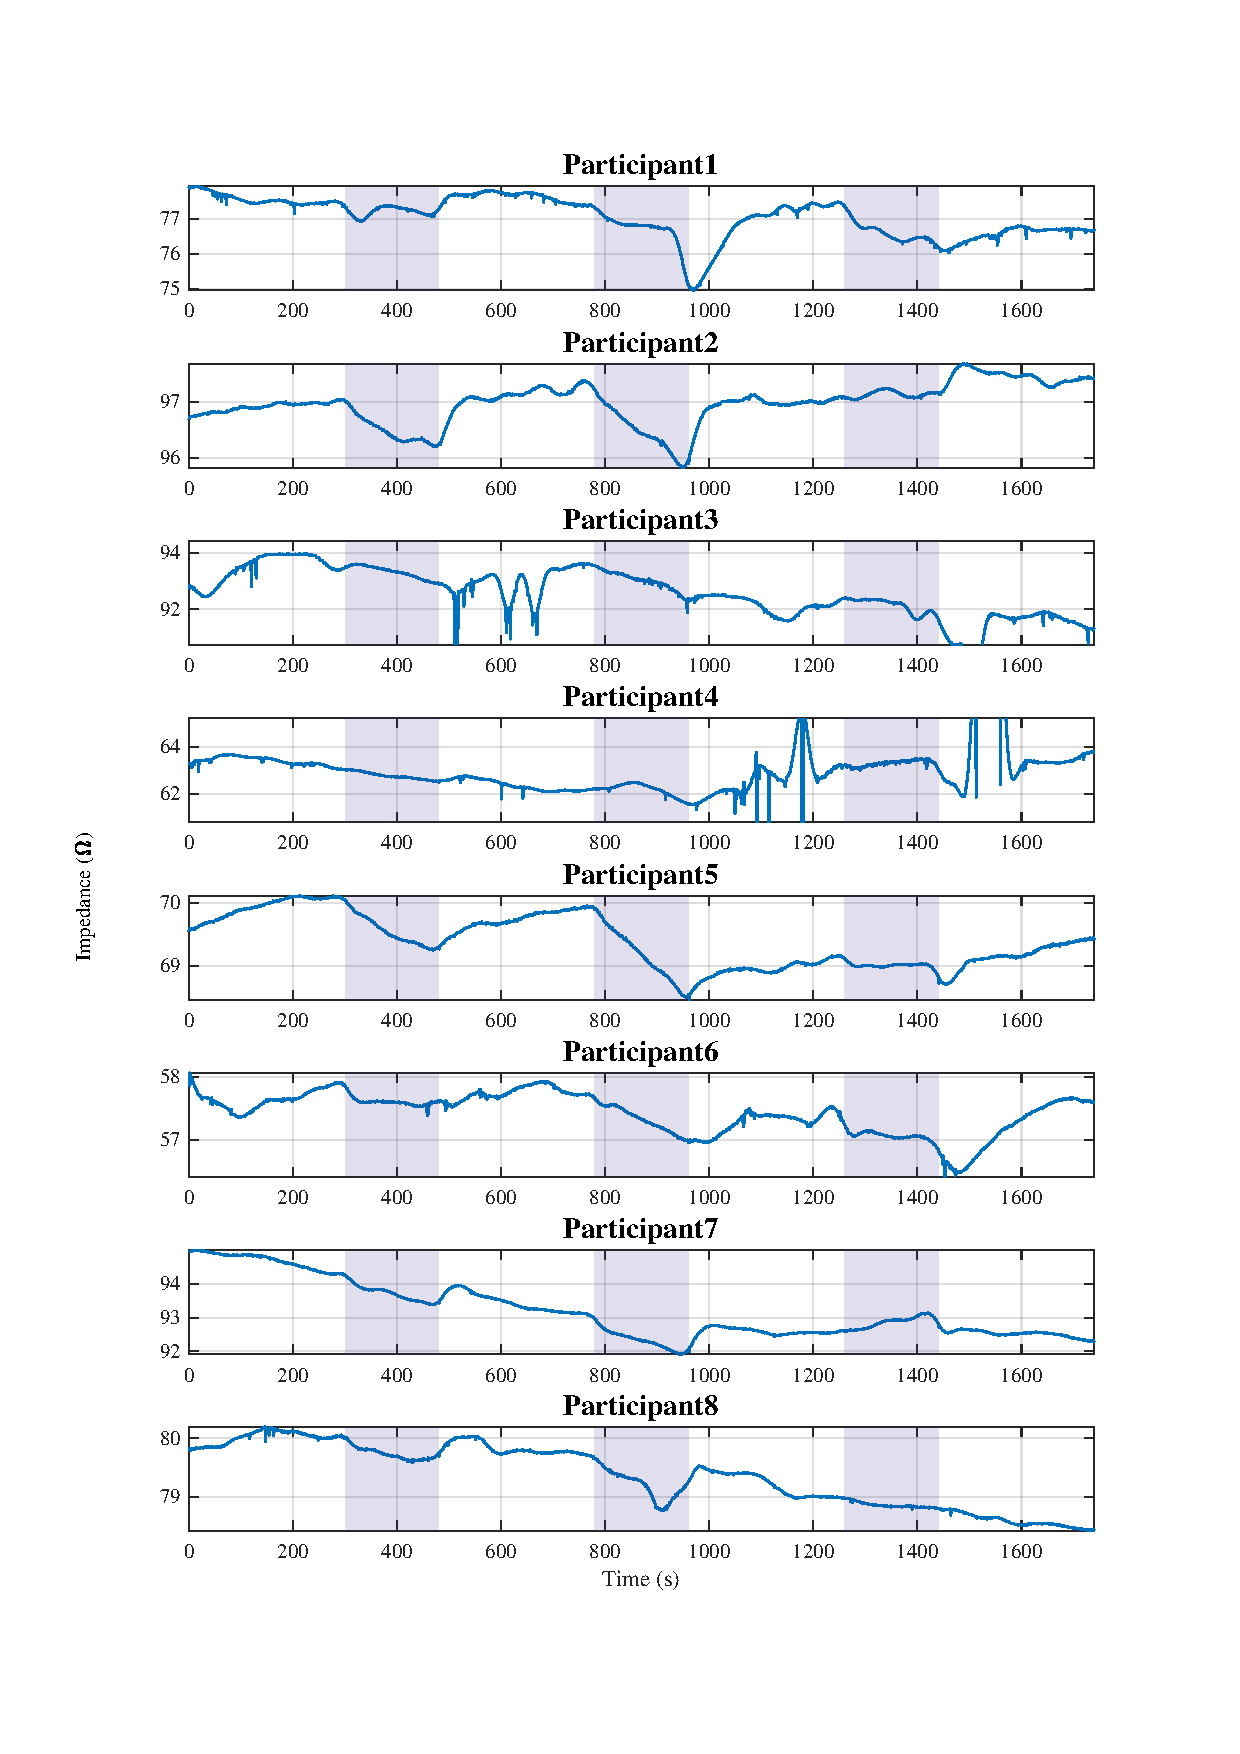
\includegraphics[width=\textwidth,height=\textheight,keepaspectratio]{figure1}    
	\caption{Baseline impedance of all the participants during the study. The shaded areas represent occlusions events.}
	\label{fig:rb:all_participants}
\end{figure}
\todo{This figure is temporary. It needs to be improved by naming axis}


%%********************************** % Section 5.1.1 ******************************************
\subsection{Basal impedance}
\label{section5.1.1}
The iPG device recorded the impedance during the first five minutes of data logging. As described in the previous chapters\todo{Maybe add a reference of the past chapter}, this signal is composed of the base impedance value and the AC waveform signal that is present with it. Moreover, this mean value is known as basal impedance, which it is equivalent to the value $R_B$ described by Nyober's equation \ref{eq:Nyober}. In other words, it is the value of the impedance before the circulation passes through the potential sensors. It is composed basically of the impedance contribution of bone, muscle, fat, skin and residual blood within the vessels. 

The device was able to detect the forearm's segment impedance quite remarkably. The values obtained felt within the resistive value estimated by the literature \todo{Find some papers with results about the impedance of the forearms}. The table \ref{tbl:basal_impedace:region1} describes the basal impedance during the first five minutes of data. 

\begin{table}[b]
	\caption{Basal impedance during the first five minutes of data with statistical values.}
	\label{tbl:basal_impedace:region1}
	
	\centering
	\begin{tabular}		
	{
	l
	c
	S[table-format=2.2]@{\,\( \pm \)\,}S[table-format=1.2] %Format for Z+-std
	*{3}{S[table-format=2.2]} 
	}
		\toprule
		              & \textbf{Size} & \multicolumn{2}{c}{\textbf{Mean [\si{\ohm}]}} & \textbf{Max [\si{\ohm}]} & \textbf{Min [\si{\ohm}]} \\ \midrule
			Participant 1  &  278  &  77.59  &  0.17  &  78.04  &  77.37\\
			Participant 2  &  295  &  96.97  &  0.09  &  97.17  &  96.76\\
			Participant 3  &  275  &  93.54  &  0.50  &  94.06  &  92.44\\
			Participant 4  &  329  &  63.44  &  0.19  &  63.77  &  63.02\\
			Participant 5  &  288  &  69.97  &  0.17  &  70.20  &  69.56\\
			Participant 6  &  331  &  57.68  &  0.17  &  58.21  &  57.33\\
			Participant 7  &  340  &  94.72  &  0.24  &  95.05  &  94.27\\
			Participant 8  &  353  &  80.04  &  0.11  &  80.30  &  79.82\\ \bottomrule
	\end{tabular} 
\end{table} 

There are different aspects of the geometry that could affect the impedance reading. There have been several studies where has been demonstrated how the distance between electrodes affects readings\todo{Add reference to studies impedance vs. length}. In the current study showed that impedance was influenced by the forearm's circumference, as well as the distance between the potential electrodes. Figure \ref{fig:C_vs_Z} indicates that there is an inverse relation between circumference and impedance. The smallest the forearm's circumference higher the resistivity. On the other hand, there is a direct relation between the distance between the potential electrodes and the resistivity of the segment as depicted in \ref{fig:l_vs_Z}.

\begin{figure*}[t!]
	\centering
	\begin{subfigure}[t]{0.5\textwidth}
		\centering
		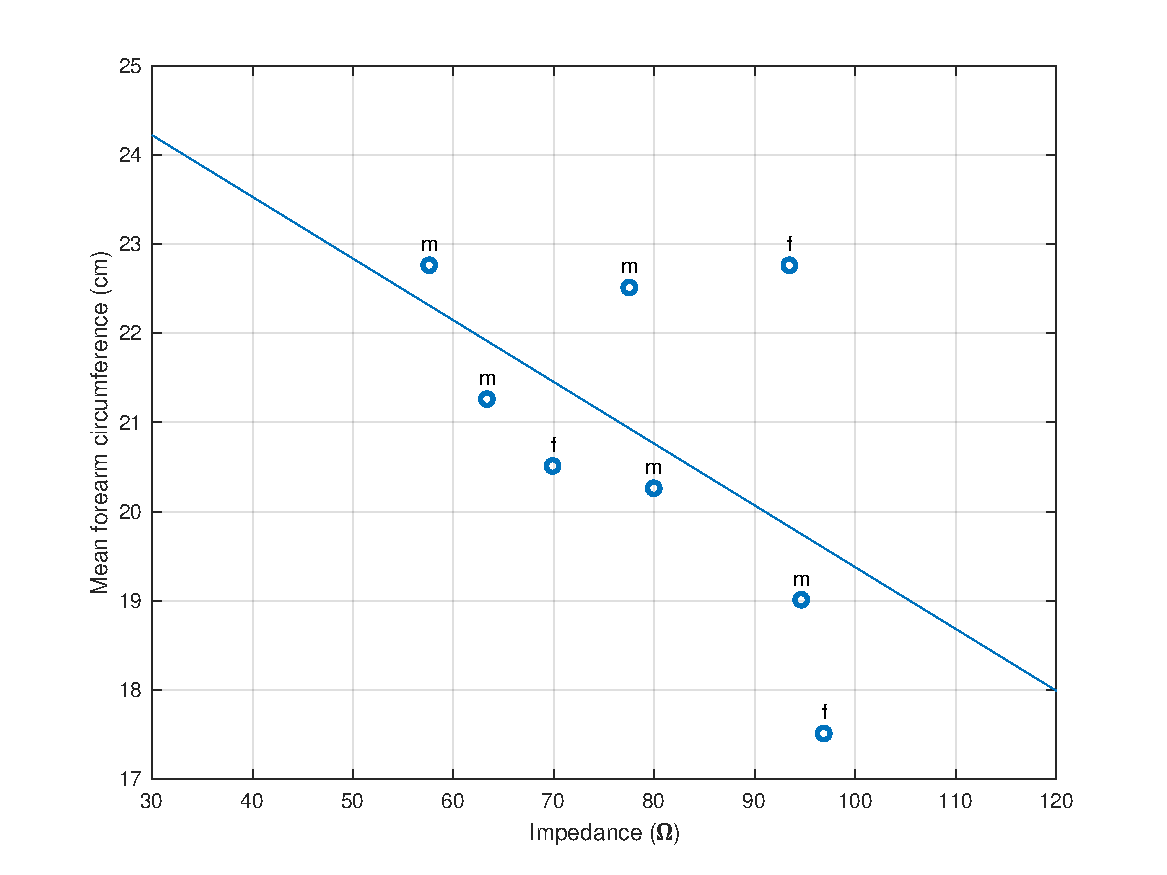
\includegraphics[height=4.5cm]{figure2a}
		\caption{Relation forearm circumference against basal impedance}
		\label{fig:C_vs_Z}
	\end{subfigure}%
	~ 
	\begin{subfigure}[t]{0.5\textwidth}
		\centering
		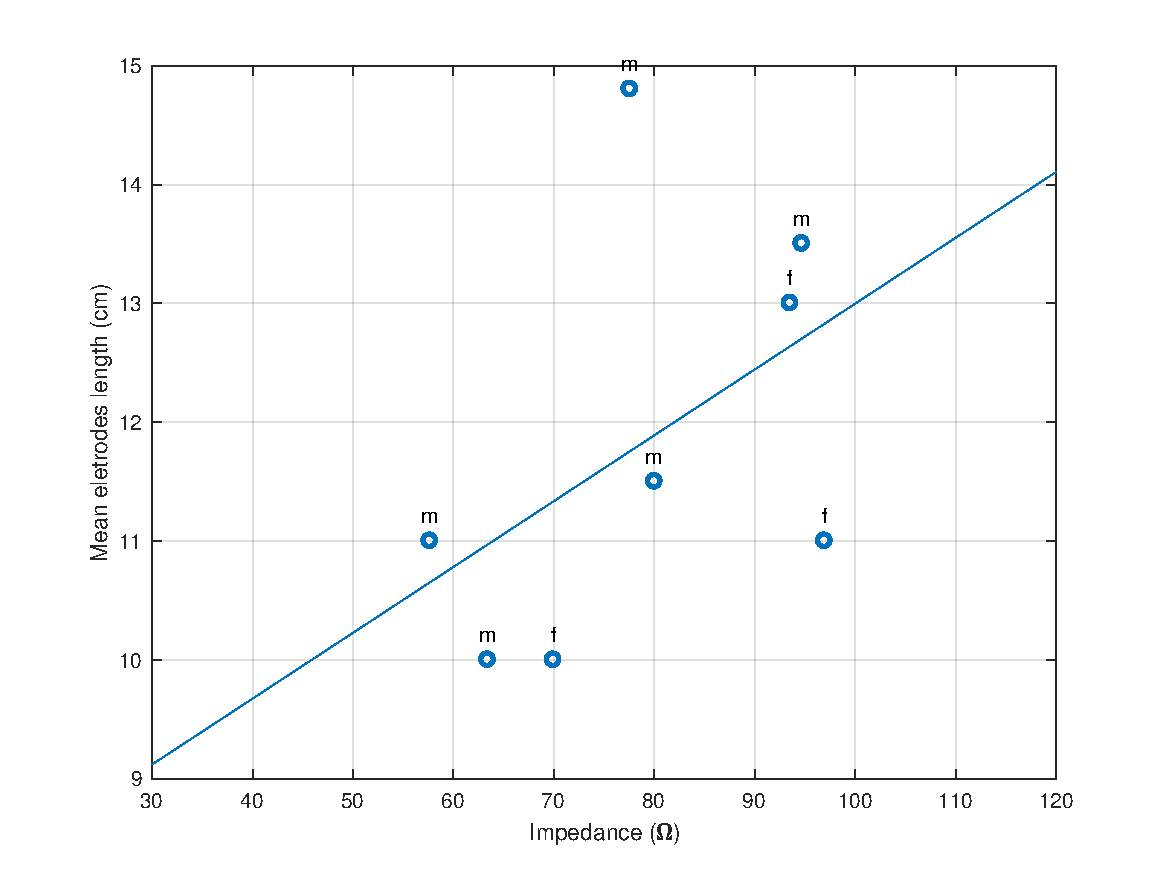
\includegraphics[height=4.5cm]{figure2b}
		\caption{Relation distance sensing electrodes against basal impedance}
		\label{fig:l_vs_Z}
	\end{subfigure}
	\caption{Relation between circumference and length affects basal impedance}
	\label{fig:relation_geometry_vs_impedance}
\end{figure*}


%%********************************** % Section 5.1.2 ******************************************
\subsection{Impedance during venous occlusion}
\label{section5.1.2}
During the following three minutes after the impedance, venous occlusion occurred. As it can be seen in figure \ref{fig:rb:all_participants} all the participants experienced a decrease in basal impedance during this time. Most of the helpers presented a linear impedance decrease trend during the occlusion. However, some of the measurements were clearly affected by motion artefact. Participants one and six are an example of this. 

In participant one, resistance fell off immediately the occlusion occurred. Nevertheless, after a minute the patron moved his arm correcting the trend. Then, impedance continued the trend again. Furthermore,  participant six also showed similar response when the arm moved. 

Figure \ref{fig:normalise:venous_occlusion} describes how the impedance behaved during the occlusion for all participants. The graph has been normalised to compare the resistivity reduction.  A linear regression was performed in the data to demonstrate the ratio of change during the occlusion.  

The table \ref{tbl:venous_occlusion:region2} overviews the results obtained from the linear regression. The value $Z_1$ illustrates the value of the impedance as the blockage started and $Z_{end}$ the resistance value at the end of the test.  $\Delta Z$ (mean $-0.632 \Omega \pm0.068\Omega$) is the variation of impedance during the \SI{3}{\minute} that the experiment last.  The slope demonstrates how much resistance is changing during each beat  (mean $-0.00271\Omega\textrm{/s}\pm3.415e^{-6}\Omega\textrm{/s}$). 

\begin{figure}
	\centering
	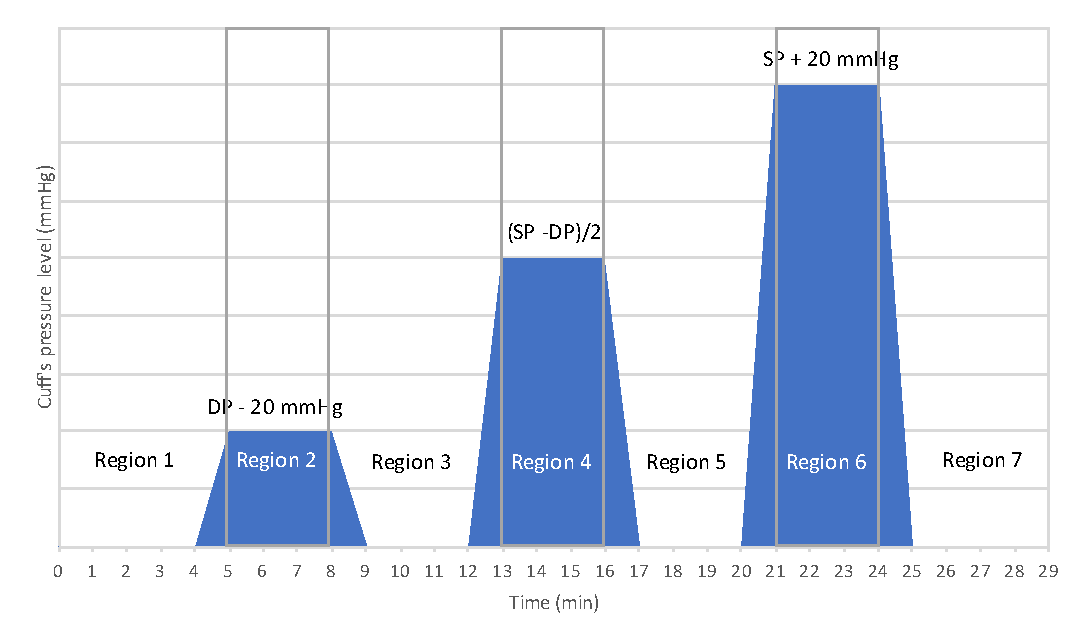
\includegraphics[width=0.9\textwidth,height=0.9\textheight,keepaspectratio]{figure3}    
	\caption{Normalise plot of impedance decrease during venous occlusion.}
	\label{fig:normalise:venous_occlusion}
\end{figure}
\todo{Figure \ref{fig:normalise:venous_occlusion} is temporary. It needs to be improved by naming axis}

\begin{table}
	\caption{Linear regression result for all participants during venous occlusion.}
	\label{tbl:venous_occlusion:region2}
	\centering
	\begin{tabu}{lcccccc}
		\toprule
		              & \textbf{Slope [\si{\ohm/\second}]} & \textbf{Intercept [\si{\ohm}]} & \textbf{$R^2$} & \textbf{$Z_1$ [\si{\ohm}]} & \textbf{$Z_{end}$ [\si{\ohm}]} & \textbf{ $\Delta Z$ [\si{\ohm}]} \\ \midrule
		Participant 1  &   0.00057  &  77.02   &     0.037  &  77.49  &  77.18  &  -0.31\\
		Participant 2  &  -0.00395  &  98.09   &     0.867  &  97.16  &  96.21  &  -0.95\\
		Participant 3  &  -0.00421  &  95.01   &     0.917  &  93.47  &  92.89  &  -0.58\\
		Participant 4  &  -0.00296  &  63.96   &     0.920  &  63.22  &  62.61  &  -0.61\\
		Participant 5  &  -0.00427  &  71.26   &     0.936  &  70.10  &  69.27  &  -0.83\\
		Participant 6  &  -0.00085  &  57.96   &     0.322  &  57.98  &  57.57  &  -0.40\\
		Participant 7  &  -0.00427  &  95.42   &     0.934  &  94.33  &  93.34  &  -0.98\\
		Participant 8  &  -0.00173  &  80.43   &     0.752  &  80.07  &  79.68  &  -0.39\\ \bottomrule
	\end{tabu} 
\end{table}

From the statistical analysis displayed can be concluded the following. First, as it was explained before, the slopes from participants 1 and 6 were affected by the motion artefact. Nevertheless, these trends seemed corrected after one minute of recordings (\SI{360}{\second}). Their slopes were quite far away from the mean value (\SI{-0.00271}{\ohm / \second}). On the other hand, the rest of the signals showed a similar trend. \todo{Review this paragraph. It seems to be very similar to the previous one.}

%********************************** % Section 5.2 ******************************************
\section{Blood flow calculation during venous occlusion}
\label{section5.2}
Using the method venous occlusion plethysmography is possible to calculate the blood flow in the forearm segment. As it can be seen from figure \ref{fig:blood_flow:venous_occlusion} the data is not dropping in a completely straight line. As a reminder, the occlusion occurred during \SIrange{300}{480}{\second} which is the time lapse showed. There are impedance variations caused by respiration movement contained within the signals, but also some sections are affected by muscle contraction. If the blood flow was computed using point by point method, there would be some discrepancies when the resistivity is increasing. Thus, this will lead to an incorrect reflection of the blood stream. 

As a result, the method described in section xxx was used to calculate the blood flow between decreasing points only. In short, this algorithm finds the peak and valleys of the signal and then computes the blood flow using equation \ref{eq:QL} between those points found. The figure \ref{fig:blood_flow:venous_occlusion} on the left shows the impedance decrease during the occlusion for all participants. The image on also depicts the points from where the algorithm extracted the reference points for its calculations. In this case, the red triangle pointing downwards is equivalent to the base impedance $R_B$ and the black triangle is the ending point of the calculation point. Then $\Delta R / \Delta t$ can be obtained as the difference between these two points in impedance and time. 
\todo{Add a section describing how the data was treated.} 

In the same figure but on the right, it can be noticed the result of the blood flow calculated in units of \si{\ml / \min 100 \ml}. The blue dots indicate the instant blood flow at the end value of $\Delta R$. The orange line indicates the mean blood flow during measurements. Again, participants 1 and 6 flow estimation is affected by movement producing a mean value far from the majority of the data points. Moreover, it is confirmed by examining the results summarised on the table \ref{tbl:blood_flow:region2}. The standard deviation $(\sigma_x)$ is quite far compared to the rest of the participants, as well as the minimum value of the data. Therefore, the results of these two participants clearly cannot be expected to be accurate. However, if the data sample was in a linear section, then the calculated flow will be more in agreement with the expected values. 

From this table can be noticed that the calculated blood flow per \SI{100}{\ml} of tissue for all the participants was in average \SI{-0.855}{\ml / \min 100\ml} $\pm$ \SI{0.344}{\ml/\min 100\ml}. 

\begin{table}[t]
	\caption{Statistics of the blood flow calculated during venous occlusion. All the numbers are in blood flow units \si{\ml/\min 100\ml}, except the column size that is the magnitude of sample.}
	\label{tbl:blood_flow:region2}
	\centering
	\begin{tabular}
		{
		l
		c
		c
		S[table-format=1.3]@{\,\( \pm \)\,}S[table-format=1.3] %Format for Z+-std 
		c
		c
		}
		\toprule
		                & \textbf{Size} & \textbf{Median} & \multicolumn{2}{c}{\textbf{Mean}} & \textbf{Max} & \textbf{Min} \\
		                & 			    & \small{\si{[\ml/\min 100\ml]}} & \multicolumn{2}{c}{\small{\si{[\ml/\min 100\ml]}}} & \small{\si{[\ml/\min 100\ml]}} & \small{\si{[\ml/\min 100\ml]}} \\\midrule
		Participant 1   & 23   &     -0.808  &   -1.055  &  0.939 &   -0.054   &  -3.955\\
		Participant 2   & 30   &     -0.570  &  -0.575   & 0.272  &  -0.117    & -1.256\\
		Participant 3   & 31   &     -0.600  &  -0.613   & 0.344  &  -0.011    & -1.483\\
		Participant 4   & 34   &     -1.131  &  -1.146   & 0.720  &  -0.016    & -2.979\\
		Participant 5   & 23   &     -0.606  &  -0.611   & 0.345  &  -0.062    & -1.737\\
		Participant 6   & 29   &     -0.710  &  -1.510   & 2.639  &  -0.092    &-10.865\\
		Participant 7   & 25   &     -0.575  &  -0.613   & 0.284  &  -0.025    & -1.141\\
		Participant 8   & 42   &     -0.605  &  -0.716   & 0.530  &  -0.072    & -2.743\\ \bottomrule
	\end{tabular} 
\end{table}


\begin{figure}
	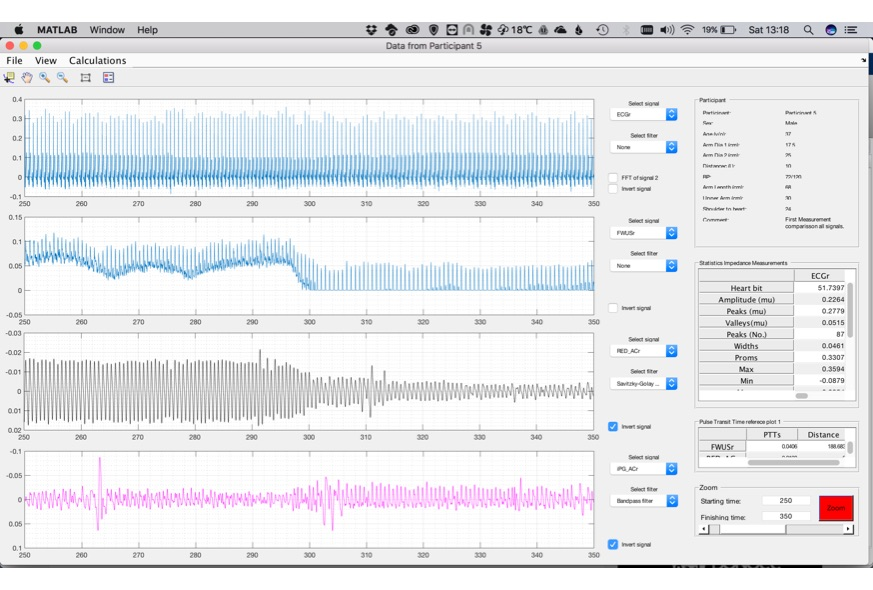
\includegraphics[width=\textwidth,height=\textheight,keepaspectratio,trim={0.5cm 0.5cm 2cm 2cm},clip]{figure4}    
	\caption{Blood flow calculated from venous occlusion plethysmography}
	\label{fig:blood_flow:venous_occlusion}
\end{figure}

